\documentclass[10pt,onecolumn,twoside,letterpaper]{article}
\usepackage[text={7in,9.5in},centering]{geometry}
\usepackage[spanish,es-nodecimaldot]{babel}

\usepackage{hyperref}

\usepackage{multicol}

\usepackage{harvard}% bibliographystyle: apsr, agsm, dcu, kluwer, nederlands

\usepackage{graphicx}
\usepackage{amssymb}
\usepackage{fancyhdr}
\usepackage{color}
\usepackage{colortbl}
\definecolor{gray}{cmyk}{0.0,0.0,0.0,0.60}

%\usepackage{auto-pst-pdf}
%\usepackage{pst-all}

%\usepackage[numbered]{mcode}
%\usepackage{lipsum}

\pagestyle{fancy}
\fancyhf{}
\fancyhead[RO]{\small{\textcolor{gray}{\textsc{Hacia un framework de locomoci\'on b\'ipeda evolutiva y flexible}}}}
\fancyhead[LO]{
\includegraphics[scale=0.05]{../../images/unlogo.png}}
\fancyhead[LE]{
\includegraphics[scale=0.05]{../../images/unlogo.png}\quad\small{\textcolor{gray}{\textsc{Linea de investigaci\'on: Robotica Evolutiva en Caminadores}}}}
\fancyfoot[CO,CE]{\thepage}
\fancyfoot[LO,RE]{\scriptsize{\textcolor{gray}{\emph{Version 0.2}}}}

\title{\vspace{-0.8cm}
\includegraphics[scale=0.12]{../../images/unescudobn.png}\\\vspace{-0.0cm}
  \LARGE \textbf{CPGs y patrones de locomoci\'on b\'ipeda}}
\author{J.A. Castillo-Le\'on\thanks{jacastillol@unal.edu.co} \and R.E. Ram\'irez-Heredia\thanks{reramirezh@unal.edu.co}}
\date{}

\begin{document}
\maketitle
\begin{abstract}\small
  Este trabajo est\'a enfocado a la implementaci\'on de una simulaci\'on de control bio-inspirado basado en CPGs, se requiere conocimiento de programaci\'on en MATLAB, fundamentos de mec\'anica y control, conceptos b\'asicos de ANNs, FLSs y GAs. 
\end{abstract}
%\begin{multicols}{2}
\section{Descripci\'on:}
Una gran tendencia actual sobre la locomoci\'on, esta siendo observada por los CPG, (\emph{Central Pattern Generators}), la cual ha permitido el control de las estructuras mec\'anicas, sin la necesidad de un modelo real de la estructura y del entorno, con gran adaptabilidad y robustez \cite{Verdaasdonk2009}.
\section{Objetivo:}
Se debe implementar mediante simulaci\'on en MATLAB, el modelo y el CPG (ver Figura \ref{fig:modelos} a y b ). Los detalles de los CPGs, se pueden encontrar en \cite{Kim2009}. Se entrega modelo del Compass-Gait en MATLAB.
%\end{multicols}
\begin{figure}[!ht]
  \centering
  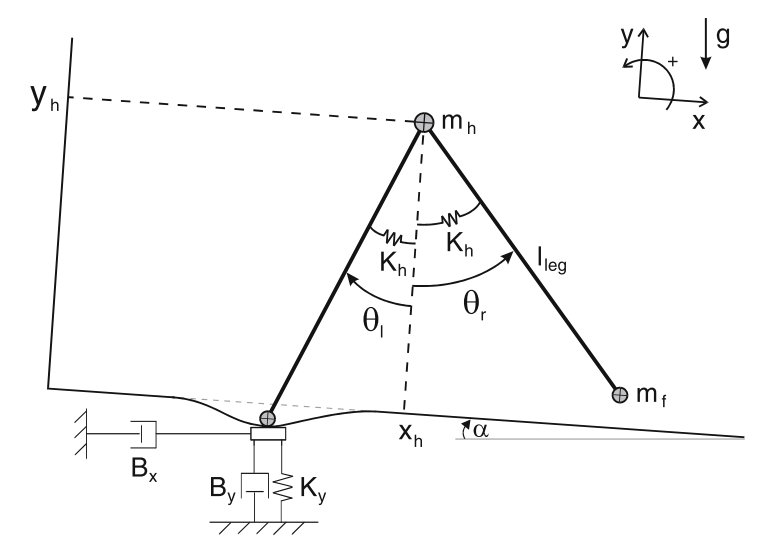
\includegraphics[scale=0.2]{../../images/VerdaasdonkCompassGaitModel.png}
  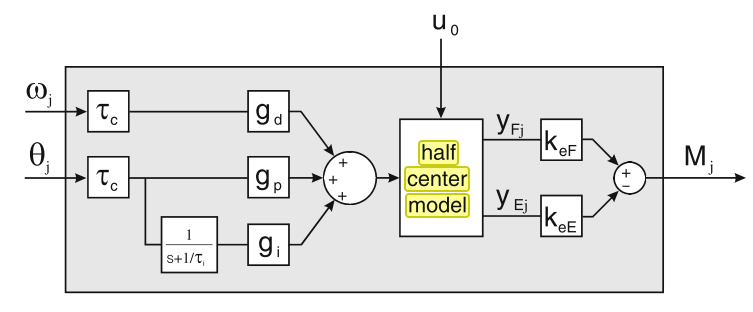
\includegraphics[scale=0.2]{../../images/VerdaasdonkCPGmodel.png}
  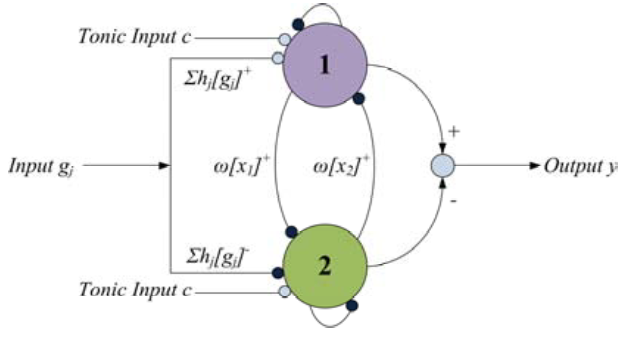
\includegraphics[scale=0.2]{../../images/KimNeuralOscillatorModel.png}\\a)\hspace{5cm}b)\hspace{4cm}c)
  \caption{\small a) Modelo Compass-Gait\protect, b) Modelo CPG-PID\protect\cite{Verdaasdonk2009} y c) Modelo Neuro-Oscilador\protect\cite{Kim2009}}
  \label{fig:modelos}
\end{figure}
%\nocite{*}
\bibliographystyle{nederlands}% apsr, agsm, dcu, kluwer, nederlands
\bibliography{../../review/review/library}
\end{document}
